\documentclass[11pt,a4paper]{report}
\usepackage[textwidth=37em,vmargin=30mm]{geometry}
\usepackage{calc,xunicode,amsmath,amssymb,paralist,enumitem,tabu,booktabs,datetime2,xeCJK,xeCJKfntef,listings}
\usepackage{tocloft,fancyhdr,tcolorbox,xcolor,graphicx,eso-pic,xltxtra,xelatexemoji}

\newcommand{\envyear}[0]{2025}
\newcommand{\envdatestr}[0]{2025-02-15}
\newcommand{\envfinaldir}[0]{webdb/2025/20250215/final}

\usepackage[hidelinks]{hyperref}
\hypersetup{
    colorlinks=false,
    pdfpagemode=FullScreen,
    pdftitle={Web Digest - \envdatestr}
}

\setlength{\cftbeforechapskip}{10pt}
\renewcommand{\cftchapfont}{\rmfamily\bfseries\large\raggedright}
\setlength{\cftbeforesecskip}{2pt}
\renewcommand{\cftsecfont}{\sffamily\small\raggedright}

\setdefaultleftmargin{2em}{2em}{1em}{1em}{1em}{1em}

\usepackage{xeCJK,xeCJKfntef}
\xeCJKsetup{PunctStyle=plain,RubberPunctSkip=false,CJKglue=\strut\hskip 0pt plus 0.1em minus 0.05em,CJKecglue=\strut\hskip 0.22em plus 0.2em}
\XeTeXlinebreaklocale "zh"
\XeTeXlinebreakskip = 0pt


\setmainfont{Brygada 1918}
\setromanfont{Brygada 1918}
\setsansfont{IBM Plex Sans}
\setmonofont{JetBrains Mono NL}
\setCJKmainfont{Noto Serif CJK SC}
\setCJKromanfont{Noto Serif CJK SC}
\setCJKsansfont{Noto Sans CJK SC}
\setCJKmonofont{Noto Sans CJK SC}

\setlength{\parindent}{0pt}
\setlength{\parskip}{8pt}
\linespread{1.15}

\lstset{
	basicstyle=\ttfamily\footnotesize,
	numbersep=5pt,
	backgroundcolor=\color{black!5},
	showspaces=false,
	showstringspaces=false,
	showtabs=false,
	tabsize=2,
	captionpos=b,
	breaklines=true,
	breakatwhitespace=true,
	breakautoindent=true,
	linewidth=\textwidth
}






\newcommand{\coverpic}[2]{
    % argv: itemurl, authorname
    Cover photo by #2~~(\href{#1}{#1})
}
\newcommand{\makeheader}[0]{
    \begin{titlepage}
        % \newgeometry{hmargin=15mm,tmargin=21mm,bmargin=12mm}
        \begin{center}
            
            \rmfamily\scshape
            \fontspec{BaskervilleF}
            \fontspec{Old Standard}
            \fontsize{59pt}{70pt}\selectfont
            WEB\hfill DIGEST
            
            \vfill
            % \vskip 30pt
            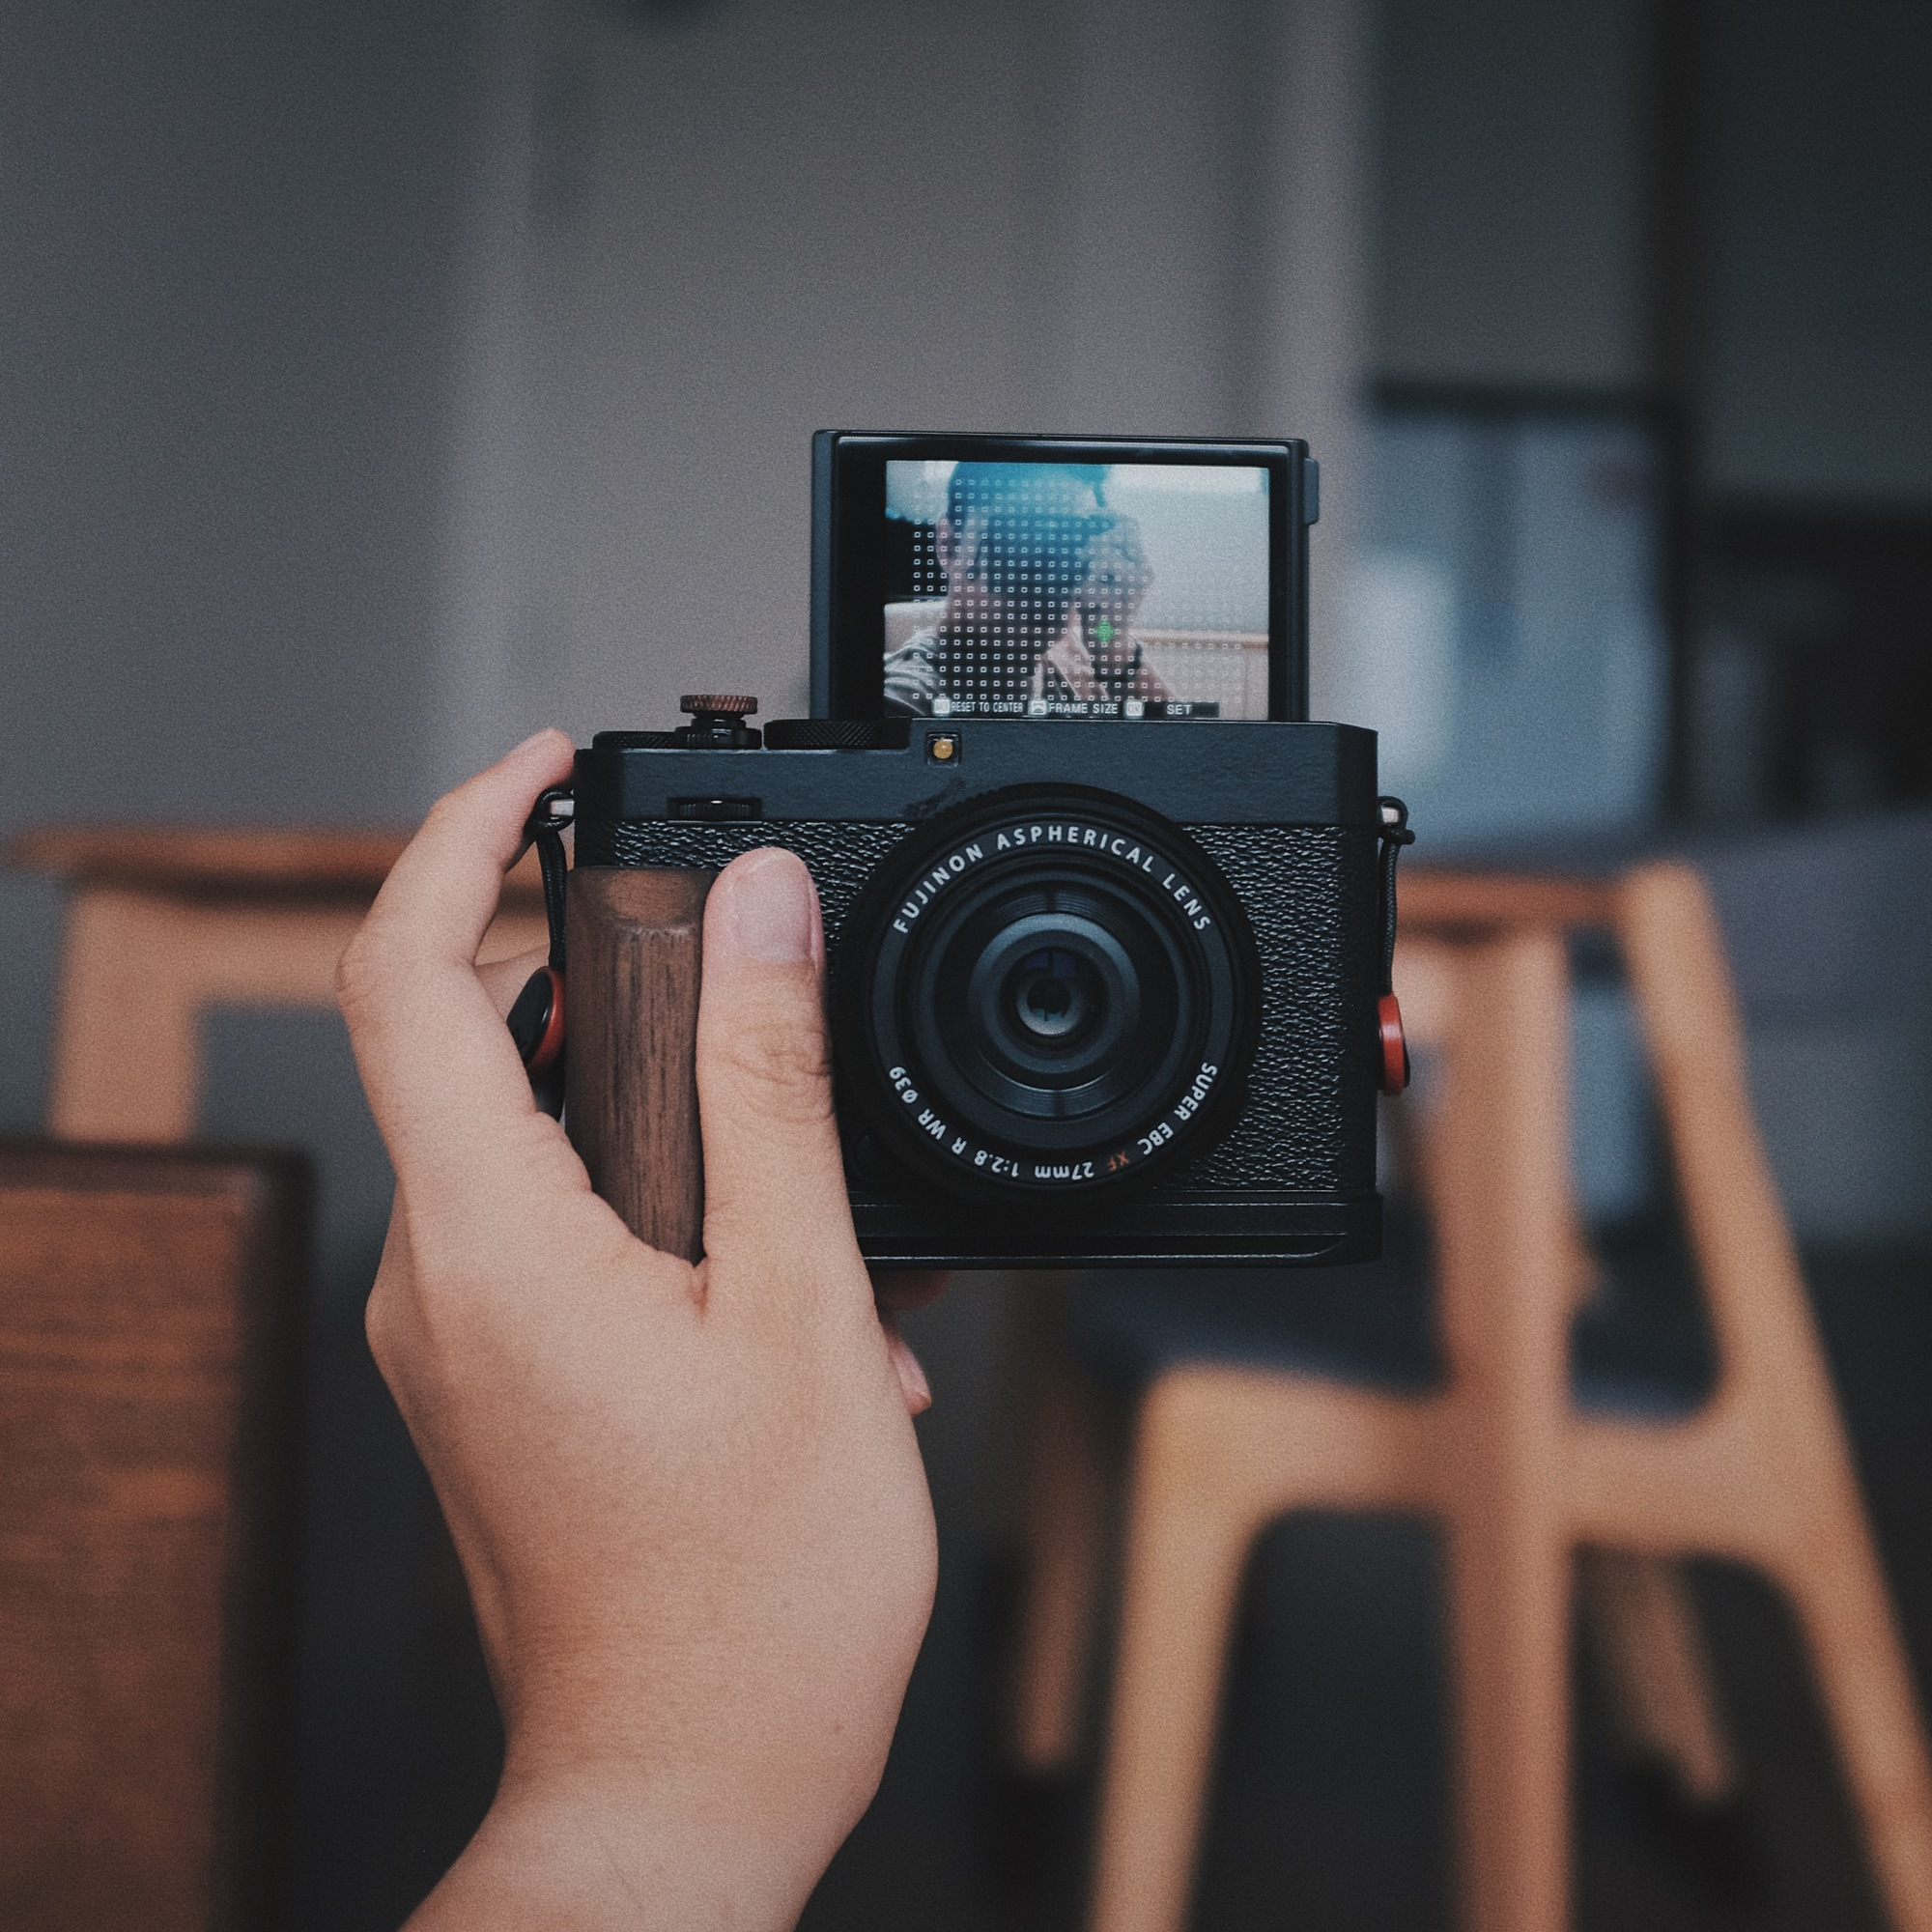
\includegraphics[width=\linewidth]{\envfinaldir/coverpic-prod.jpg}\par
            % \vskip 30pt
            \vfill

            \normalsize\rmfamily\scshape
            \copyright{} The Web Digest Project \hfill\large \envdatestr
        \end{center}
    \end{titlepage}
    % \restoregeometry
}
\newcommand{\simplehref}[1]{%
    \textcolor{blue!80!green}{\href{#1}{#1}}%
}
\renewcommand{\contentsname}{\center\Huge\sffamily\bfseries Contents\par\vskip 20pt}
\newcounter{ipartcounter}
\setcounter{ipartcounter}{0}
\newcommand{\ipart}[1]{
    % \vskip 20pt
    \clearpage
    \stepcounter{ipartcounter}
    \phantomsection
    \addcontentsline{toc}{chapter}{#1}
    % \begin{center}
    %     \Huge
    %     \sffamily\bfseries
    %     #1
    % \end{center}
    % \vskip 20pt plus 7pt
}
\newcounter{ichaptercounter}
\setcounter{ichaptercounter}{0}
\newcommand{\ichapter}[1]{
    % \vskip 20pt
    \clearpage
    \stepcounter{ichaptercounter}
    \phantomsection
    \addcontentsline{toc}{section}{\numberline{\arabic{ichaptercounter}}#1}
    \begin{center}
        \Huge
        \sffamily\bfseries
        #1
    \end{center}
    \vskip 20pt plus 7pt
}
\newcommand{\entrytitlefont}[1]{\subsection*{\raggedright\Large\sffamily\bfseries#1}}
\newcommand{\entryitemGeneric}[2]{
    % argv: title, url
    \parbox{\linewidth}{
        \entrytitlefont{#1}\par\vskip 5pt
        \footnotesize\ttfamily\mdseries
        \simplehref{#2}
    }\vskip 11pt plus 11pt minus 1pt
}
\newcommand{\entryitemGithub}[3]{
    % argv: title, url, desc
    \parbox{\linewidth}{
        \entrytitlefont{#1}\par\vskip 5pt
        \footnotesize\ttfamily\mdseries
        \simplehref{#2}\par\vskip 5pt
        \small\rmfamily\mdseries#3
    }\vskip 11pt plus 11pt minus 1pt
}
\newcommand{\entryitemAp}[3]{
    % argv: title, url, desc
    \parbox{\linewidth}{
        \entrytitlefont{#1}\par\vskip 5pt
        \footnotesize\ttfamily\mdseries
        \simplehref{#2}\par\vskip 5pt
        \small\rmfamily\mdseries#3
    }\vskip 11pt plus 11pt minus 1pt
}
\newcommand{\entryitemHackernews}[3]{
    % argv: title, hnurl, rawurl
    % \parbox{\linewidth}{
    %     \entrytitlefont{#1}\par\vskip 5pt
    %     \footnotesize\ttfamily\mdseries
    %     \simplehref{#3}\par
    %     \textcolor{black!50}{\href{#2}{#2}}
    % }\vskip 11pt plus 11pt minus 1pt
    \begin{minipage}{\linewidth}
            \entrytitlefont{#1}\par\vskip 5pt
            \footnotesize\ttfamily\mdseries
            \simplehref{#3}\par
            \textcolor{black!50}{\href{#2}{#2}}
    \end{minipage}\par\vskip 11pt plus 11pt minus 1pt
}







\begin{document}

\makeheader

\tableofcontents\clearpage




\ipart{Developers}
\ichapter{Hacker News}
\entryitemTwoLinks{We Were Wrong About GPUs}{https://news.ycombinator.com/item?id=43053844}{https://fly.io/blog/wrong-about-gpu/}

\entryitemTwoLinks{LinkedIn is the worst social media I've ever seen}{https://news.ycombinator.com/item?id=43052409}{https://news.ycombinator.com/item?id=43052409}

\entryitemTwoLinks{Kevin Mitnik FOIA Final}{https://news.ycombinator.com/item?id=43051802}{https://vault.fbi.gov/kevin-mitnick/kevin-mitnick-part-01-final/view}

\entryitemTwoLinks{Delphi Is 30}{https://news.ycombinator.com/item?id=43051598}{https://blog.marcocantu.com/blog/2025-february-delphi-is-30.html}

\entryitemTwoLinks{A study on how turtles navigate using the Earth's magnetic field}{https://news.ycombinator.com/item?id=43051465}{https://www.unc.edu/posts/2025/02/12/dancing-turtles-unlock-scientific-discovery/}

\entryitemTwoLinks{Detecting AI agent use and abuse}{https://news.ycombinator.com/item?id=43049959}{https://stytch.com/blog/detecting-ai-agent-use-abuse/}

\entryitemTwoLinks{DA, sheriff, who shared woman's nude photos on phone are covered by QI}{https://news.ycombinator.com/item?id=43049174}{https://www.oregonlive.com/crime/2025/02/an-oregon-womans-nude-cellphone-photos-ended-up-the-talk-of-town-she-tracked-it-back-to-the-da.html}

\entryitemTwoLinks{ICE wants to know if you're posting negative things about it online}{https://news.ycombinator.com/item?id=43049152}{https://theintercept.com/2025/02/11/ice-immigration-social-media-surveillance/}

\entryitemTwoLinks{The History of S.u.S.E}{https://news.ycombinator.com/item?id=43048261}{https://www.abortretry.fail/p/the-history-of-suse}

\entryitemTwoLinks{Show HN: Transform your codebase into a single Markdown doc for feeding into AI}{https://news.ycombinator.com/item?id=43048027}{https://tesserato.web.app/posts/2025-02-12-CodeWeaver-launch/index.html}

\entryitemTwoLinks{Watchdog ponders why Apple doesn't apply its strict app tracking rules to itself}{https://news.ycombinator.com/item?id=43047952}{https://www.theregister.com/2025/02/14/apple\_app\_tracking\_probe/}

\entryitemTwoLinks{AI is stifling new tech adoption?}{https://news.ycombinator.com/item?id=43047792}{https://vale.rocks/posts/ai-is-stifling-tech-adoption}

\entryitemTwoLinks{"Homotopical macrocosms for higher category theory" identified as woke DEI grant}{https://news.ycombinator.com/item?id=43046466}{https://mathstodon.xyz/@johncarlosbaez/114000054766059217}

\entryitemTwoLinks{Linux kernel cgroups writeback high CPU troubleshooting}{https://news.ycombinator.com/item?id=43046174}{https://dasl.cc/2025/01/01/debugging-our-new-linux-kernel/}

\entryitemTwoLinks{Anyone can push updates to the doge.gov website}{https://news.ycombinator.com/item?id=43045835}{https://www.404media.co/anyone-can-push-updates-to-the-doge-gov-website-2/}

\entryitemTwoLinks{Benchmarking vision-language models on OCR in dynamic video environments}{https://news.ycombinator.com/item?id=43045801}{https://arxiv.org/abs/2502.06445}

\entryitemTwoLinks{On Bloat}{https://news.ycombinator.com/item?id=43045713}{https://docs.google.com/presentation/d/e/2PACX-1vSmIbSwh1\_DXKEMU5YKgYpt5\_b4yfOfpfEOKS5\_cvtLdiHsX6zt-gNeisamRuCtDtCb2SbTafTI8V47/pub?start=false\&loop=false\&delayms=3000}

\entryitemTwoLinks{Extensible WASM Applications with Go}{https://news.ycombinator.com/item?id=43045698}{https://go.dev/blog/wasmexport}

\entryitemTwoLinks{Zed now predicts your next edit with Zeta, our new open model}{https://news.ycombinator.com/item?id=43045606}{https://zed.dev/blog/edit-prediction}

\entryitemTwoLinks{The New York Stock Exchange plans to launch NYSE Texas}{https://news.ycombinator.com/item?id=43045558}{https://ir.theice.com/press/news-details/2025/The-New-York-Stock-Exchange-to-Launch-NYSE-Texas/default.aspx}\ichapter{Phoronix}
\entryitemGeneric{\hskip 0pt{}Dynamic Triple Buffering Merged For GNOME 48}{https://www.phoronix.com/news/GNOME-48-Triple-Buffering}

\entryitemGeneric{\hskip 0pt{}Linux 6.15 To Ensure PlayStation 5 Controllers Use The Correct Driver}{https://www.phoronix.com/news/Linux-6.15-Ensures-PS5-Driver}

\entryitemGeneric{\hskip 0pt{}Fwupd 2.0.6 Adds Support For HPE Gen10/Gen10+ Servers}{https://www.phoronix.com/news/Fwupd-2.0.6-Released}

\entryitemGeneric{\hskip 0pt{}Ubuntu Making Progress On Replacing initramfs-tools With Dracut}{https://www.phoronix.com/news/Ubuntu-Dracut-Still-WIP}

\entryitemGeneric{\hskip 0pt{}GNOME Software May Eventually Drop RPM Support In Favor Of Flatpaks}{https://www.phoronix.com/news/GNOME-Software-RPM-Flatpak}

\entryitemGeneric{\hskip 0pt{}Show Your Love For Linux Hardware Coverage By Going Premium This Valentine's Day}{https://www.phoronix.com/news/Phoronix-Premium-Valentine-2025}

\entryitemGeneric{\hskip 0pt{}Vulkan 1.4.308 Brings NVIDIA's Provisional Present Metering Extension}{https://www.phoronix.com/news/Vulkan-1.4.308-Present-Metering}

\entryitemGeneric{\hskip 0pt{}Valkey 8.1-rc1 Delivers Fresh Performance Improvements}{https://www.phoronix.com/news/Valkey-8.1-rc1}

\entryitemGeneric{\hskip 0pt{}TrueNAS 25.04 "Fangtooth" Beta Unifies Linux SCALE \& FreeBSD CORE Efforts}{https://www.phoronix.com/news/TrueNAS-25.04-Beta}\ichapter{Dribbble}
\entryitemGeneric{\hskip 0pt{}Alpaca}{https://dribbble.com/shots/25627851-Alpaca}

\entryitemGeneric{\hskip 0pt{}Ethereum Wordmark Logo Concept}{https://dribbble.com/shots/25623390-Ethereum-Wordmark-Logo-Concept}

\entryitemGeneric{\hskip 0pt{}Illustration}{https://dribbble.com/shots/25619766-Illustration}

\entryitemGeneric{\hskip 0pt{}Carbon Solutions B2B Dashboard Design}{https://dribbble.com/shots/25554521-Carbon-Solutions-B2B-Dashboard-Design}

\entryitemGeneric{\hskip 0pt{}Love Potion}{https://dribbble.com/shots/25619714-Love-Potion}

\entryitemGeneric{\hskip 0pt{}Pirate Parrot}{https://dribbble.com/shots/25619077-Pirate-Parrot}

\entryitemGeneric{\hskip 0pt{}Mortar\&Carrot}{https://dribbble.com/shots/25619708-Mortar-Carrot}

\entryitemGeneric{\hskip 0pt{}SPROXX - LOGO DESIGN}{https://dribbble.com/shots/25619328-SPROXX-LOGO-DESIGN}

\entryitemGeneric{\hskip 0pt{}Master / God / Cloud}{https://dribbble.com/shots/25619810-Master-God-Cloud}

\entryitemGeneric{\hskip 0pt{}Fast Turn Fittings}{https://dribbble.com/shots/25619395-Fast-Turn-Fittings}

\entryitemGeneric{\hskip 0pt{}Black Cat Speed Shop®}{https://dribbble.com/shots/25614666-Black-Cat-Speed-Shop}

\entryitemGeneric{\hskip 0pt{}Fintech icons pack download}{https://dribbble.com/shots/25607159-Fintech-icons-pack-download}

\entryitemGeneric{\hskip 0pt{}Self Love}{https://dribbble.com/shots/25607914-Self-Love}

\entryitemGeneric{\hskip 0pt{}Urban Echo}{https://dribbble.com/shots/25608526-Urban-Echo}

\entryitemGeneric{\hskip 0pt{}Cloaked Wireless Device}{https://dribbble.com/shots/25403560-Cloaked-Wireless-Device}

\entryitemGeneric{\hskip 0pt{}Logo tip 001. Symmetry and asymmetry}{https://dribbble.com/shots/25606111-Logo-tip-001-Symmetry-and-asymmetry}

\entryitemGeneric{\hskip 0pt{}World Peace}{https://dribbble.com/shots/25609765-World-Peace}

\entryitemGeneric{\hskip 0pt{}Sentinal - Logo Design}{https://dribbble.com/shots/25606497-Sentinal-Logo-Design}

\entryitemGeneric{\hskip 0pt{}Tanuki}{https://dribbble.com/shots/25606258-Tanuki}

\entryitemGeneric{\hskip 0pt{}Dirty Dutch - Brand Mark / Logo}{https://dribbble.com/shots/25604523-Dirty-Dutch-Brand-Mark-Logo}

\entryitemGeneric{\hskip 0pt{}Cast AI Logo Redesign}{https://dribbble.com/shots/25607135-Cast-AI-Logo-Redesign}

\entryitemGeneric{\hskip 0pt{}Running Partners}{https://dribbble.com/shots/25606250-Running-Partners}

\entryitemGeneric{\hskip 0pt{}Recruit Management App}{https://dribbble.com/shots/25593875-Recruit-Management-App}

\entryitemGeneric{\hskip 0pt{}Logo}{https://dribbble.com/shots/25597775-Logo}


\ipart{Developers~~~~(zh-Hans)}
\ichapter{Solidot}
\entryitemGeneric{\hskip 0pt{}亚马逊将关闭 Kindle 的 Download \& Transfer via USB 功能}{https://www.solidot.org/story?sid=80564}

\entryitemGeneric{\hskip 0pt{}摩根大通 CEO 对反对重返办公室的意见不屑一顾}{https://www.solidot.org/story?sid=80563}

\entryitemGeneric{\hskip 0pt{}20 光年外的一颗恒星宜居带有行星}{https://www.solidot.org/story?sid=80562}

\entryitemGeneric{\hskip 0pt{}美摄起诉字节跳动抄袭代码获赔 8266.8 万元}{https://www.solidot.org/story?sid=80561}

\entryitemGeneric{\hskip 0pt{}俄罗斯无人机攻击切尔诺贝利核电站}{https://www.solidot.org/story?sid=80560}

\entryitemGeneric{\hskip 0pt{}Zed 使用开源模型 Zeta 预测用户的编辑}{https://www.solidot.org/story?sid=80559}

\entryitemGeneric{\hskip 0pt{}Arm 将自己制造芯片}{https://www.solidot.org/story?sid=80558}

\entryitemGeneric{\hskip 0pt{}作为换囚交易的一部分美国释放了 BTC-e 联合创始人}{https://www.solidot.org/story?sid=80557}

\entryitemGeneric{\hskip 0pt{}攻读博士学位的人数在减少}{https://www.solidot.org/story?sid=80556}

\entryitemGeneric{\hskip 0pt{}中国居民对 AI 的信任高于美国}{https://www.solidot.org/story?sid=80555}

\entryitemGeneric{\hskip 0pt{}研究发现 AI 的新闻摘要会经常性的扭曲事实}{https://www.solidot.org/story?sid=80554}

\entryitemGeneric{\hskip 0pt{}Google 和苹果恢复上架 TikTok}{https://www.solidot.org/story?sid=80553}

\entryitemGeneric{\hskip 0pt{}Google 计划用机器学习估计用户的年龄}{https://www.solidot.org/story?sid=80552}

\entryitemGeneric{\hskip 0pt{}印度儿童的心算能力不能转变学校里的数学分数}{https://www.solidot.org/story?sid=80551}

\entryitemGeneric{\hskip 0pt{}百度宣布文心一言 4 月 1 日起免费}{https://www.solidot.org/story?sid=80550}

\entryitemGeneric{\hskip 0pt{}丰田等多家日企内部禁用 DeepSeek}{https://www.solidot.org/story?sid=80549}

\entryitemGeneric{\hskip 0pt{}科学家探测到迄今最高能的中微子}{https://www.solidot.org/story?sid=80548}

\entryitemGeneric{\hskip 0pt{}大脑中的微塑料是否会伤害你?}{https://www.solidot.org/story?sid=80547}

\entryitemGeneric{\hskip 0pt{}NOAA 公开泰坦号内爆音频}{https://www.solidot.org/story?sid=80546}

\entryitemGeneric{\hskip 0pt{}汤森路透在美国赢得 AI 版权侵犯诉讼}{https://www.solidot.org/story?sid=80545}\ichapter{V2EX}
\entryitemGeneric{\hskip 0pt{}[互联网] 豆瓣不再提供电影海报的原图下载了?}{https://www.v2ex.com/t/1111597}

\entryitemGeneric{\hskip 0pt{}[生活] 现在什么都要问一下 deepseek 了}{https://www.v2ex.com/t/1111596}

\entryitemGeneric{\hskip 0pt{}[问与答] (并非日经?) 求推荐适应一些特殊需求的笔记软件}{https://www.v2ex.com/t/1111595}

\entryitemGeneric{\hskip 0pt{}[VPS] ¥ 45 出瓦工 BWG-THE DC9 PLAN CN2GIA}{https://www.v2ex.com/t/1111594}

\entryitemGeneric{\hskip 0pt{}[OpenWrt] 求助,关于 OpenWrt 的使用}{https://www.v2ex.com/t/1111593}

\entryitemGeneric{\hskip 0pt{}[Steam] 92-95 折代买任何 steam 国区游戏}{https://www.v2ex.com/t/1111591}

\entryitemGeneric{\hskip 0pt{}[问与答] 为什么 2025 年央视蛇年春晚的歌曲这么伤感,每一首歌听起来都很想哭。}{https://www.v2ex.com/t/1111590}

\entryitemGeneric{\hskip 0pt{}[分享发现] iPhone 2022 se 的 阿里 NFC 卡 可能是沉默启用的}{https://www.v2ex.com/t/1111589}

\entryitemGeneric{\hskip 0pt{}[云计算] 请问下,突发性能实例的 2u 和经济型的 2u 性能上有啥区别吗?}{https://www.v2ex.com/t/1111588}

\entryitemGeneric{\hskip 0pt{}[问与答] 14 寸 macbookpro24g+512g 的 M4 pro 和 1w 多的超薄 ROG 笔记本(i9 4070) , 哪个更好用}{https://www.v2ex.com/t/1111585}

\entryitemGeneric{\hskip 0pt{}[投资] 30 万怎么合理配置资产}{https://www.v2ex.com/t/1111581}

\entryitemGeneric{\hskip 0pt{}[分享发现] deepseek R1 官方竟然是全部开源的, 开源就是满血}{https://www.v2ex.com/t/1111580}

\entryitemGeneric{\hskip 0pt{}[分享创造] 用 JS 脚本控制你的 Android 手机}{https://www.v2ex.com/t/1111579}

\entryitemGeneric{\hskip 0pt{}[程序员] 新手小白接收 usdt,选什么钱包}{https://www.v2ex.com/t/1111576}

\entryitemGeneric{\hskip 0pt{}[生活] 父亲老烟民,冠心病,叫戒烟不听~咋办}{https://www.v2ex.com/t/1111575}

\entryitemGeneric{\hskip 0pt{}[职场话题] 请教内地上班,香港发薪问题}{https://www.v2ex.com/t/1111574}

\entryitemGeneric{\hskip 0pt{}[酷工作] [快手] [IOS] [接受安卓转 IOS] [团队直招]}{https://www.v2ex.com/t/1111573}

\entryitemGeneric{\hskip 0pt{}[职场话题] 29 岁 Fe 又提大礼包,何去何从}{https://www.v2ex.com/t/1111571}

\entryitemGeneric{\hskip 0pt{}[全球工单系统] Cloudcone 不退款}{https://www.v2ex.com/t/1111570}

\entryitemGeneric{\hskip 0pt{}[云计算] 对``服务器繁忙''说拜拜,最快最稳最便宜的 DeepSeek API!}{https://www.v2ex.com/t/1111569}

\entryitemGeneric{\hskip 0pt{}[问与答] 求推荐性价比高的人体工程学椅子}{https://www.v2ex.com/t/1111568}

\entryitemGeneric{\hskip 0pt{}[问与答] 有什么办法可以 代码实现 触发 这个元素的显示吗?}{https://www.v2ex.com/t/1111567}

\entryitemGeneric{\hskip 0pt{}[问与答] ios 佳明 connect 有替代 app 吗}{https://www.v2ex.com/t/1111566}

\entryitemGeneric{\hskip 0pt{}[生活] 广大宅男 对谈恋爱有莫大的误解}{https://www.v2ex.com/t/1111563}

\entryitemGeneric{\hskip 0pt{}[随想] 大佬表示:``绝对不要教 AI 说谎,绝对要让 AI 最大化对真理的遵循。''这个逻辑我看不懂。}{https://www.v2ex.com/t/1111561}

\entryitemGeneric{\hskip 0pt{}[问与答] email、短信、电话,发信人向收信人付费,可以实现吗?}{https://www.v2ex.com/t/1111560}

\entryitemGeneric{\hskip 0pt{}[生活] 我不生孩子的 10 个理由}{https://www.v2ex.com/t/1111559}

\entryitemGeneric{\hskip 0pt{}[全球工单系统] notion 服务器是不是炸了?}{https://www.v2ex.com/t/1111558}

\entryitemGeneric{\hskip 0pt{}[问与答] 微软 Edge 浏览器账密同步问题}{https://www.v2ex.com/t/1111557}

\entryitemGeneric{\hskip 0pt{}[Android] 咨询:如何能看应用触发的 opengl 指令数吗}{https://www.v2ex.com/t/1111555}

\entryitemGeneric{\hskip 0pt{}[生活] 这人啥心态啊?}{https://www.v2ex.com/t/1111553}

\entryitemGeneric{\hskip 0pt{}[NAS] 分享一下自己封装的 Kodi 国内镜像插件库}{https://www.v2ex.com/t/1111552}

\entryitemGeneric{\hskip 0pt{}[YouTube] 怎么下载油管 8K 视频?}{https://www.v2ex.com/t/1111550}

\entryitemGeneric{\hskip 0pt{}[职场话题] 从培训班看市场需求}{https://www.v2ex.com/t/1111549}

\entryitemGeneric{\hskip 0pt{}[求职] 求职重庆 golang | 后端}{https://www.v2ex.com/t/1111547}

\entryitemGeneric{\hskip 0pt{}[问与答] 你们有过低血糖导致虚脱吗?}{https://www.v2ex.com/t/1111545}

\entryitemGeneric{\hskip 0pt{}[程序员] AI 编辑器百花齐放, JB 家还这么落后,但是有动作了, Junie 有人进 Waitlist 了吗?}{https://www.v2ex.com/t/1111544}

\entryitemGeneric{\hskip 0pt{}[OpenAI] NextChat 里面的``面具''功能是干什么用的?}{https://www.v2ex.com/t/1111542}

\entryitemGeneric{\hskip 0pt{}[硬件] N 卡又贵又断货,买块 AMD Radeon RX 7900 XTX 凑合一下怎么样?}{https://www.v2ex.com/t/1111541}

\entryitemGeneric{\hskip 0pt{}[问与答] 大家有没有尝试过用 AI 生成代码文档?有没有推荐的,效果怎么样?}{https://www.v2ex.com/t/1111539}

\entryitemGeneric{\hskip 0pt{}[程序员] 手搓了个 Web 分析统计(Cloudflare Pages)}{https://www.v2ex.com/t/1111537}

\entryitemGeneric{\hskip 0pt{}[职场话题] 大伙在写代码时会不会迷茫?}{https://www.v2ex.com/t/1111535}

\entryitemGeneric{\hskip 0pt{}[宽带症候群] 若大的这么三个电信运营商,把正规和非正规渠道的资费差异搞成这么大}{https://www.v2ex.com/t/1111534}

\entryitemGeneric{\hskip 0pt{}[问与答] 请问大家是如何在 excel 编辑 json 单元格呢?}{https://www.v2ex.com/t/1111533}

\entryitemGeneric{\hskip 0pt{}[开源软件] 打造高效用户旅程:埋点分析系统的实操指南}{https://www.v2ex.com/t/1111532}

\entryitemGeneric{\hskip 0pt{}[PayPal] 好久没有 paypal 了,问下各位大佬}{https://www.v2ex.com/t/1111531}

\entryitemGeneric{\hskip 0pt{}[Apple] macbookpro M4 pro 京东国补现在是好时间入手吗}{https://www.v2ex.com/t/1111529}

\entryitemGeneric{\hskip 0pt{}[职场话题] 记一同事心梗去世}{https://www.v2ex.com/t/1111528}

\entryitemGeneric{\hskip 0pt{}[投资] 50w,当下比较稳健的理财方式和途径有哪些?}{https://www.v2ex.com/t/1111526}

\entryitemGeneric{\hskip 0pt{}[生活] 老婆更喜欢给猫添置物品}{https://www.v2ex.com/t/1111524}


\ipart{Generic News}
\ichapter{AP News}
\entryitemWithDescription{\hskip 0pt{}Philadelphia turns green on Valentine's Day to celebrate Super Bowl champions}{https://apnews.com/article/13a0ef26a02b9a8405bc09a1b1eb37d8}{}

\entryitemWithDescription{\hskip 0pt{}A humpback whale briefly swallows kayaker in Chilean Patagonia — and it's all captured on camera}{https://apnews.com/article/b0cafde4b640326f20a9da28003d6c26}{}

\entryitemWithDescription{\hskip 0pt{}Many Americans think Valentine's Day is romantic and fun — not outdated or stressful: AP-NORC poll}{https://apnews.com/article/ed8022bbc4726c02800e410ea88e5a8a}{}

\entryitemWithDescription{\hskip 0pt{}Prosecutor at A\$AP Rocky trial tells jurors they can't consider his partner Rihanna or their kids}{https://apnews.com/article/854d3a4d79934148069b7ffcc45556d4}{}

\entryitemWithDescription{\hskip 0pt{}Man whose wife was killed in a hippo attack in Africa sues the US company that booked the trip}{https://apnews.com/article/620d0109bf84a7765f489f83e4f116ae}{}

\entryitemWithDescription{\hskip 0pt{}Why asteroid 2024 YR4 is unlikely to hit Earth in 2032}{https://apnews.com/article/5c353e2ee53bb1ecd68a562611d54062}{}

\entryitemWithDescription{\hskip 0pt{}Some people didn't know they had a bird flu infection, study of veterinarians suggests}{https://apnews.com/article/e468e1dec4c4344c4719f0b23be00540}{}

\entryitemWithDescription{\hskip 0pt{}US aircraft carrier Truman collides with merchant ship near Egypt, but no injuries are reported}{https://apnews.com/article/50e039f339c4658d246a08ca496a21d9}{}

\entryitemWithDescription{\hskip 0pt{}Darkly hilarious fundraisers allow those scorned by love a little revenge for Valentine's Day}{https://apnews.com/article/40537881d8f5ad65dd971fef11a856f5}{}

\entryitemWithDescription{\hskip 0pt{}Archaeologists unearth the remains of a Roman basilica on the site of a new London skyscraper}{https://apnews.com/article/38df5698485f50bfc00c487b1fb246ec}{}

\entryitemWithDescription{\hskip 0pt{}A rare photo shows Russian and American fighter jets in one place, in India}{https://apnews.com/article/4df9323e2f4a05a4182d1c1cbdbe0573}{}

\entryitemWithDescription{\hskip 0pt{}A fire at Buddhist temple in New York killed 2 people, including a monk}{https://apnews.com/article/aec537024512e570e01261e67b77bf78}{}

\entryitemWithDescription{\hskip 0pt{}Saudi educator known for charity and prisoner work wins \$1 million Global Teacher Prize}{https://apnews.com/article/12b222f6ae1698c0ce580e2c01f3baa6}{}\ichapter{Reuters}
\entryitemWithDescription{\hskip 0pt{}Trump backs 'hard stance' on Gaza, says he does not know what Israel will do}{https://www.reuters.com/world/trump-backs-hard-stance-gaza-says-he-does-not-know-what-israel-will-do-2025-02-14/}{President Donald Trump on Friday advocated taking a "hard stance" on Gaza, the Palestinian enclave for which he has proposed a U.S. takeover and where a fragile ceasefire between Israel and Palestinian Hamas militants is in...}

\entryitemWithDescription{\hskip 0pt{}Trump funding freeze halts wildfire prevention work}{https://www.reuters.com/world/us/trump-funding-freeze-halts-wildfire-prevention-work-2025-02-14/}{The Trump administration has halted funding for federal programs to reduce wildfire risk in Western states and has frozen hiring of seasonal firefighters, as part of broad cuts to government spending, according to organizations impacted...}

\entryitemWithDescription{\hskip 0pt{}Trump keeps tariffs drumbeat going, with autos targeted next}{https://www.reuters.com/business/trump-keeps-tariffs-drumbeat-going-with-autos-targeted-next-2025-02-14/}{President Donald Trump on Friday kept alive his drumbeat of tariff threats, saying levies on automobiles would be coming as soon as April 2, the day after members of his cabinet are due to deliver reports to him outlining options for a...}

\entryitemWithDescription{\hskip 0pt{}UN peacekeeping mission outgoing deputy force commander injured after convoy attacked in Beirut}{https://www.reuters.com/world/middle-east/un-peacekeeping-mission-outgoing-deputy-force-commander-injured-after-convoy-2025-02-14/}{The outgoing deputy force commander of the United Nations Interim Force in Lebanon (UNIFIL) was injured on Friday after a convoy taking peacekeepers to Beirut airport was "violently attacked," UNIFIL...}

\entryitemWithDescription{\hskip 0pt{}EU's Kallas calls foreign ministers' meeting to talk about US, Ukraine}{https://www.reuters.com/world/eus-kallas-calls-foreign-ministers-meeting-talk-about-us-ukraine-2025-02-14/}{European Union foreign policy chief Kaja Kallas has invited foreign ministers from the bloc attending the Munich Security Conference to meet on Sunday to discuss relations with the Trump administration and the war in...}

\entryitemWithDescription{\hskip 0pt{}Vance meets with leader of German far-right AfD party}{https://www.reuters.com/world/vance-meets-with-leader-german-far-right-afd-party-2025-02-14/}{U.S. Vice President JD Vance met on Friday with Alice Weidel, the leader of the far-right Alternative for Germany (AfD) party, while on a visit to Germany, an official in Vance\textquotesingle s office said, according to a pool...}

\entryitemWithDescription{\hskip 0pt{}Russian drone attack damaged Chornobyl plant's confinement structure, chief engineer says}{https://www.reuters.com/world/europe/russian-drone-attack-damaged-chornobyl-plants-confinement-structure-chief-2025-02-14/}{A Russian drone attack badly damaged the confinement structure around the disused Chornobyl nuclear power plant intended to prevent the release of nuclear substances, a senior nuclear industry official said on...}

\entryitemWithDescription{\hskip 0pt{}US probing 'bad data' possibly used by Black Hawk crew before deadly crash, official says}{https://www.reuters.com/world/us/us-probing-bad-data-possibly-used-by-black-hawk-crew-before-deadly-crash-2025-02-14/}{The National Transportation Safety Board is examining "bad data" the crew of an Army Black Hawk helicopter may have relied upon prior to its deadly crash with a passenger jet outside Washington D.C. late last month, an official...}

\entryitemWithDescription{\hskip 0pt{}Top US, Philippine diplomats discussed South China Sea, economic cooperation, State Dept says}{https://www.reuters.com/world/top-us-philippine-diplomats-discussed-south-china-sea-economic-cooperation-state-2025-02-14/}{U.S. Secretary of State Marco Rubio and Philippine Foreign Minister Enrique Manalo, in a meeting in Munich on Friday, discussed bilateral coordination in the South China Sea and increasing economic cooperation, the State Department...}

\entryitemWithDescription{\hskip 0pt{}Trump says he agreed to meet UK's Starmer in next few weeks}{https://www.reuters.com/world/trump-says-he-agreed-meet-uks-starmer-next-few-weeks-2025-02-14/}{U.S. President Donald Trump said on Friday that he had spoken with British Prime Minister Keir Starmer the day before and he agreed to meet with him, perhaps in the next few...}

\entryitemWithDescription{\hskip 0pt{}Approval rating of Brazil's Lula falls to 24\% from 35\%, pollster Datafolha says}{https://www.reuters.com/world/americas/brazils-lula-approval-rating-falls-24-35-pollster-datafolha-says-2025-02-14/}{Approval of Brazilian President Luiz Inacio Lula da Silva\textquotesingle s government dropped to 24\% from 35\% in December, pollster Datafolha said on...}

\entryitemWithDescription{\hskip 0pt{}Exclusive: US global disaster response teams unable to deploy following USAID shutdown, sources say}{https://www.reuters.com/world/us/us-disaster-response-teams-unable-deploy-following-usaid-shutdown-sources-say-2025-02-14/}{A world-renowned U.S. program for international disaster and crisis assistance can no longer deploy in the event of a major emergency due to the Trump administration\textquotesingle s dismantling of the U.S. foreign aid agency, nine...}

\entryitemWithDescription{\hskip 0pt{}New traces of tear gas found on Ukraine battlefield by chemical weapons watchdog}{https://www.reuters.com/world/europe/new-traces-tear-gas-found-ukraine-battlefield-by-chemical-weapons-watchdog-2025-02-14/}{The world\textquotesingle s chemical weapons watchdog on Friday said it had once again found traces of tear gas on the frontline with Russia in Ukraine\textquotesingle s central-east Dnipropetrovsk...}






\clearpage
\leavevmode\vfill
\footnotesize

Copyright \copyright{} 2023-2025 Neruthes and other contributors.

This document is published with CC BY-NC-ND 4.0 license.

The entries listed in this newsletter may be copyrighted by their respective creators.

This newsletter is generated by the Web Digest project.

The newsletters are also delivered via Telegram channel \CJKunderline{\href{https://t.me/webdigestchannel}{https://t.me/webdigestchannel}}.\\
RSS feed is available at \CJKunderline{\href{https://webdigest.pages.dev/rss.xml}{https://webdigest.pages.dev/rss.xml}}.

This newsletter is available in PDF at
\CJKunderline{\href{https://webdigest.pages.dev/}{https://webdigest.pages.dev/}}.

The source code being used to generate this newsletter is available at\\
\CJKunderline{\href{https://github.com/neruthes/webdigest}{https://github.com/neruthes/webdigest}}.

This newsletter is also available in
\CJKunderline{\href{http://webdigest.pages.dev/readhtml/\envyear/WebDigest-20250215.html}{HTML}} and
\CJKunderline{\href{https://github.com/neruthes/webdigest/blob/master/markdown/\envyear/WebDigest-20250215.md}{Markdown}}.


\coverpic{https://unsplash.com/photos/a-black-and-white-photo-of-a-person-standing-on-a-beach-JN33B7MWj84}{Gin Majka}


\end{document}
